\section{Question 11.4}

\subsection{Question}
Show how the linear feature-based ranking function is related to the abstract ranking model from Chapter 5.


\subsection{Answer}
Starting with the first mention of the abstract ranking model in the textbook, refer to Figure \ref{fig:51}.  This is an example of the abstract ranking model for a single document.

\begin{figure}[H]
\centering
\label{fig:51}
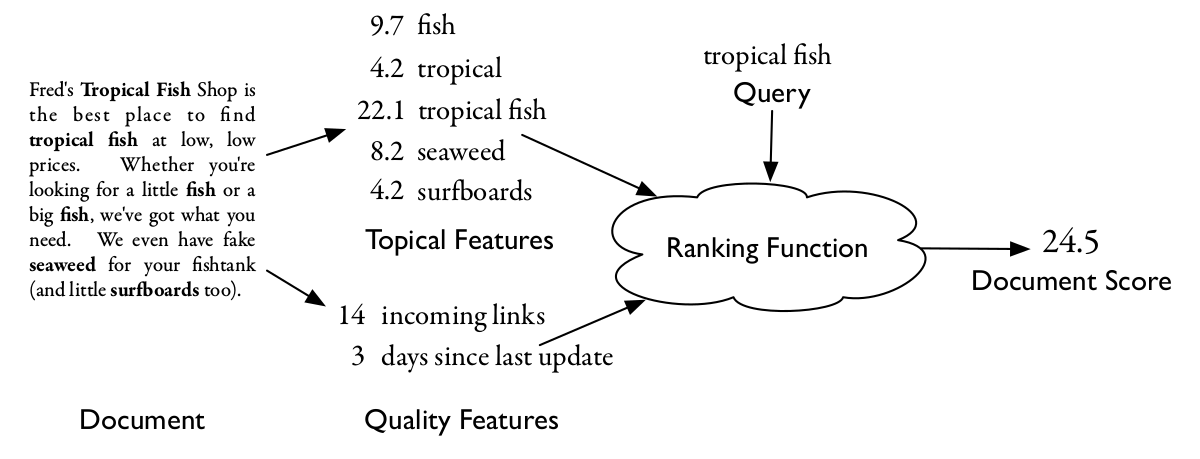
\includegraphics[scale=.25]{q11.4/fig51.png}
\caption{The components of the abstract model of ranking\dots}
\end{figure}

A more formal definition can be found in equation \ref{eq:1}:

\begin{equation}
\label{eq:1}
R(Q, D) = \sum_i g_i (Q) f_i (D)
\end{equation}

This is a linear combination of two feature functions: \(f_i\) extracts a score from the document and \(g_i\) extracts a score from the query.\\

Now, for a definition of the linear feature-based retrieval model, refer to Equation \ref{eq:2}:

\begin{equation}
\label{eq:2}
S_\Lambda(D;Q) = \sum_j \lambda_j \cdot f_j(D, Q) + Z
\end{equation}

here, \(f_j\) is a feature function that extracts a score from query/document pairs, \(\lambda_j \in \Lambda\) are parameters, and \(Z\) is a constant.  This is also a linear combination of functions that emit scores, which is similar to how the abstract ranking model works, with the addition of the parameters (\(\Lambda\)) and constant (\(Z\)).